\section{Methodology}
%DESCRIBE HOW WE GATHER AND TIME BASIC BLOCKS 
\subsection{Basic Block Collection}
We selected the source applications of our basic blocks with two goals:
\begin{enumerate*}
    \item The set of applications should cover a diverse range
of domains to represent real world workload
    \item Their basic blocks should reflect input that concerns typical users of a performance model;
    compiler developers deals with
    basic blocks from general purpose programs,
    which have different characteristics
    than those from 
    high performance kernels. 
\end{enumerate*}

We selected Clang/LLVM\cite{llvm} (compiler),
Redis (in-memory database), SQLite (database), and Gzip (compression)
to collect basic blocks that represent
applications that are written in general purpose languages
like C and C++.
Basic blocks from these programs
typically have high memory traffic, and are usually not-vectorized.
We chose these applications because they are some of the mostly used
applications today; they are well tuned for performance;
and they all have sophisticated use of algorithms and data structures,
giving us a large source of diverse basic blocks.

We selected high performance kernels from the following domains:
cryptography (OpenSSL), scientific computing (OpenBLAS),
machine learning (TensorFlow\cite{tensorflow}),
and rendering/multimedia (Embree\cite{embree} and FFmpeg).
All aforementioned applications --
with the exception of TensorFlow and Embree -- 
have kernels written in assembly.
Embree is written in ispc\cite{ispc}, a data parallel language
designed specifically to target Intel's vector extensions.

We collected basic blocks from these applications using
a dynamic analysis implemented in DynamoRIO\cite{dynamorio},
which provides an API to record every basic block
executed at runtime.
We opted for dynamic analysis rather than static disassembly
because precise static disassembly of x86 binary
is undecidable.
We use the official benchmark suites of these applications\footnote{
Except for FFmpeg and Gzip, which to the best of our knowledge do not have
official benchmarks. For these two applications we use inputs
from https://openbenchmarking.org.
} to simulate realistic execution of these applications when performing
the dynamic analysis.

\subsection{Timing Infrastructure}
We now describe our approach to profiling basic block thoughput.
We use IACA's definition of throughput, i.e. 
the average number of cycles required to execute a basic block inside
an infinite loop.
We guarantee the following invariants for our measurements.
\begin{itemize}
\item All memory data reside in L1 cache.
This is what tools like llvm-mca and IACA assume.

\item Measurements should be free of interrupts, context switches,
and hyper-threading.
\end{itemize}

\textbf{Deriving throughput from latency}.
The basic strategy one usually takes to measure basic block throughput
is unrolling a basic block multiple times and divide the latency of the
unrolled basic block by the unroll factor.
Compared to running the basic block inside a loop,
unrolling has an advantage in that the measurement is not polluted by
the overhead incurred by looping.
A typical unroll factor is 100\cite{ithemal,uops}.
Such a high unroll factor can however incur significant
L1-icache misses for large basic blocks
(e.g. already unrolled inner-loop body of a GEMM kernel).
The issue with unrolling naively is that,
an unroll-factor small enough to fit the 
unrolled basic block into instruction cache is on the other hand
insufficient to hide the latency of the first few iterations.
We thus adopted a different strategy to cope with large basic blocks.

We unroll each basic block with two different unroll factors.
These factors should be large enough 
to warm-up the processor into steady state.
We then measure the latency of the two unrolled basic blocks,
calculate the difference in latency, and divide it 
by difference of the unroll factors.
The resulting number is the throughput of the basic block.
Consider a processor that enters steady state
after executing a basic block 10 iterations.
We measure the latency of this basic block expanded with
two unroll factors -- 10 and 20.
Suppose the resulting latency is 120 and 200 respectively,
we can then determine that the throughput of this basic block
is $\frac{200-120}{20-10} = 8$ cycles per iteration.

\textbf{Handling memory accesses}.
Consider the basic block in figure \ref{fig:mem-ex},
which is used to compute the CRC code of input bytes in Gzip.
Highlighted instructions shows flow of pointer values;
essentially \textit{bits} of \verb|rdx| are used to index into a lookup table, 
and the content of which is then used in the next iteration to 
update \verb|rdx|.
How would one profile the throughput of this basic block?
Without the original application context,
this basic block \textit{cannot} be directly executed.
Developer of Gzip familiar with this piece of code could 
setup a micro-benchmark properly by reproducing the
relevant lookup table used by this code snippet,
but such approach would not scale to the hundred of 
thousands of basic blocks in our data set, most of which contain memory accesses.
We needed some way to automatically generate the benchmarking environment
without apriori knowledge/assumption of the code being profiled.

\begin{figure}[h]
\begin{Verbatim}[commandchars=\#\{\}]
    add rdi, 1
    #hl{mov eax, edx}
    shr rdx, 8
    #hl{xor al, [rdi - 1]}
    movzx eax, al
    #hl{xor rdx, [8*rax + 0x4110ah0]}
    cmp rdi, rcx
\end{Verbatim}
\caption{Inner loop body of updcrc from Gzip.
This basic block cannot be directly executed because
of its memory accesses.}
\label{fig:mem-ex}
\end{figure}
%TODO: point out concretely why previous approach, including prefixing
% addresses with the array does not work

A possible solution\cite{ithemal} is rewriting
the basic block so that all memory accesses are
relative to a pre-allocated array.
For instance, \verb|mov [rdx], 1| is rewritten to
\verb|mov [addr_of_arr+rdx], 1|. 
This approach has several issues.
\begin{itemize}
    \item Executing some basic blocks back to back can result in a 
    diverging (e.g. strided) access pattern. 
    One would need to pre-allocate an unrealistically large array
    in order to  accommodate for this pattern, 
    Even when a sufficiently large buffer could be allocated,
    this access pattern can result in cache misses, 
    which we want to avoid.
    \item The rewriting scheme does not take stack accesses
    into account.
    \item Rewritten instructions can
    have larger encoding, which can affect throughput
    of front-end bound basic blocks.
\end{itemize}

We avoid these pitfalls with a new technique
that divides the profiling process into two stages:
\begin{enumerate*}
\item We profile the virtual pages accessed by
the basic block (were it to run without crashing)
and map those pages to a single physical page.
\item After the appropriate mappings are created,
the unrolled basic block is then executed normally under
the new page mapping.
\end{enumerate*}

\textbf{Page Mapping}. 
In addition to legalizing all memory accesses made by the basic block,
the mapping stage also ensures that all memory accesses stay in
the L1 cache.
Mapping is done by executing the unrolled basic block in a forked process
 monitored by a parent process using \verb|ptrace|.
Each attempt to access an unmapped virtual page is intercepted by
the monitoring process, which then instructs the 
executing process to create the appropriate mapping
and to restart execution from the \textit{beginning}
with all registers, memory values,
as well as flag registers reinitialized.
Re-initialization is done to ensure that in the final measurement
stage the trace of memory addresses computed by the 
unrolled basic block is \textit{identical} to that from the mapping stage.

We make additional optimizations to further
increase our chance of successfully obtaining clean measurements.
Prior to the mapping-run,
we unmap all pages (except those containing the basic block).
This allows us to run basic blocks that inadvertently
writes to library code such as libc.
The physical page is
always initialized to be filled with a “moderately sized” constant
(we used \verb|0x12345600| in our experiments)
to accommodate for indirect memory accesses.
To see why this is necessary,
consider a basic block that first loads a pointer $p$ from memory
and then de-references $p$.
If the value of $p$ is too low (e.g. 0)
or too high
(i.e. bigger than the maximum memory that
a user space program is allowed to addressed),
then we will not be able to map the virtual page pointed by $p$.

\textbf{Handling Subnormal Numbers}.
General speaking -- aside from division
and specialized instructions such as \verb|sqrt|
-- floating point instructions have constant timing
except when input of the operations are subnormal numbers.
In our experiments where we encountered subnormal numbers,
floating point operations can be slowed down by up to 20x.
To ``normalize'' our timing, we configured \verb|MXCSR| register
to disable gradual underflow.

\textbf{Avoiding context switches and interrupts}.
The execution phase of profiling is done in kernel mode
to avoid performance fluctuation incurred by context switches
and interrupts.
This is implemented as a kernel driver that executes
user-supplied function pointer in kernel mode.
Preemptions and interrupts are disabled during measurement.

One might ask, were all the precautions we took in profiling necessary?
Table \ref{tab:ablation} shows the effect of incrementally applying
different optimizations to remove measurement noise.
Without some of our optimizations, the measurement could be 
two orders of magnitude off in the worst case.

\begin{table}
\begin{tabular}{
|p{0.2\columnwidth}|p{0.18\columnwidth}|p{0.18\columnwidth}|p{0.18\columnwidth}|}
\hline (Additional) Optimizations &
Measured Throughput &
L1 D-Cache Misses &
L1 I-Cache Misses \\

\hline
None & Crashed & N/A & N/A \\

\hline
Page mapping & 6377.0 & 956 & 0 \\

\hline
Single physical page & 2273.7 & 0 & 0 \\

\hline
Disabling gradual underflow & 65.0 & 0 & 35 \\

\hline
Using smaller unroll factor & 59.0 & 0 & 0\\

\hline
\end{tabular}
\\
\caption{Measured throughput for a sample basic block when
different measurement optimizations are incrementally applied.
The basic block is extracted from one of the critical 
inner loop body of TensorFlow\cite{tensorflow}'s CNN training benchmark.}
\label{tab:ablation}
\end{table}


\subsection{Basic Block Classifications}\label{classification}
Our benchmark reports the accuracy of a performance model in two modes:
\begin{enumerate*}
\item Weighted error for each application
\item Average prediction error of different classes of 
basic blocks (e.g. performance prediction
of basic blocks in numerical kernels vs.
cryptographic kernels).
\end{enumerate*}

\textbf{Per-application error}.
We collected program counter samples
in our dynamic analysis.
Using this information, we are able to weight each basic block by
the approximate frequency with which it is executed during runtime.
Weighting the basic blocks allows us to focus on basic blocks that have
non-negligible effects on performance.
Most basic blocks collected from TensorFlow\cite{tensorflow},
for instance, are from infrequently executed code 
such as the Python interpreter or glibc;
weighting these basic blocks allows a user of the benchmark
to see an evaluation the performance model relevant
to the application's expected runtime cost.

\textbf{Per-class error}. 
We automatically classify the basic blocks into
to different categories.
The high-level approach we took was to first,
\begin{enumerate*}
\item map each basic block to a vector representation
that reflects its usage of hardware resources,
\item and then cluster the basic blocks by their vector representations.
\end{enumerate*}

Using results from Abel and Reineke\cite{uops},
we compute a port-combination mapping for each instruction.
For instance,
the port-combination mapping for \verb|xor rax, rbx| in Haswell
is $\{ p0156 \rightarrow 1 \}$ (using Abel and Reineke's notation);
in other words, this instruction is implemented 
with a micro-op that can be executed at port-0, 5, and 6.
In Haswell, there are 13 such port combinations for all userland instructions.
Accordingly, we create a 13-element vector for each instruction such that
the $i'$th element denotes the number of micro-ops can be executed
on the $i'$th port-combination.
Similarly, we compute a 13-element vector for each basic block
in our dataset by summing over the port-combination vectors
of all instructions in the basic block and normalizing the vector by 
the total number of micro-ops.

After obtaining vector representation for the basic blocks, 
we used K-means\cite{kmeans} to partition the basic blocks into 20 clusters.
Table \ref{tab:clusters} gives a brief summary of the superficial characteristics
of each cluster; as the summary suggests, our clustering has semantic meaning.
We settled on using 20 clusters to balance
the tradeoff between the uniqueness of each cluster
and similarity of basic blocks within the same cluster;
using less clusters caused multiple partitions to have
near identical distributions of basic blocks,
and using too many grouped dissimilar basic blocks together.
Figure\ref{fig:apps_vs_clusters} shows the breakdown of each applications
by the classification of its basic blocks.
\begin{table}
\begin{tabular}{|p{0.15\columnwidth}|p{0.6\columnwidth}|p{0.1\columnwidth}|}
    \hline
    Cluster & Description & Size \\
    \hline
    
    Cluter-1 & 
    Loads mixed with few ALU ops & 49873 \\
    \hline
    
    Cluster-2 &
    Stores mixed with few ALU ops & 13062 \\
    \hline
    
    Cluster-3 &
    Memory ops with stores on the heavy side & 12804 \\
    \hline
    
    Cluster-4 &
    Memory ops with loads on the heavy side & 8042 \\
    \hline
    
    Cluster-5 &
    ALU ops & 12344 \\
    \hline
    
    Cluster-6 &
    ALU ops sprinkled with memory ops & 11735 \\
    \hline
    
    Cluster-7 &
    Loads & 33318 \\
    \hline
    
    Cluster-8 &
    Stores sprinkled with ALU ops & 18262 \\
    \hline
    
    Cluster-9 &
    Loads & 15826 \\
    \hline
    
    Cluster-10 &
    Vector instructions & 1378 \\
    \hline
    
    Cluster-11 &
    Non-memory \verb|mov|s and \verb|lea|s & 26744 \\ 
    \hline
    
    Cluster-12 &
    Mix of loads and stores & 12419 \\
    \hline
    
    Cluster-13 &
    ALU sprinkled with loads & 3930 \\
    \hline
    
    Cluster-14 &
    ALU ops & 51213 \\
    \hline
    
    Cluster-15 &
    ALU (more \verb|mul|s, \verb|divs|, and shifts compared to Cluster-14) & 3035 \\
    \hline
    
    Cluster-16 &
    Vectorized instructions & 914 \\
    \hline
    
    Cluster-17 &
    Memory ops dominated by loads & 16665 \\
    \hline
    
    Cluster-18 &
    Vectorized code with little memory traffic & 494 \\
    \hline
    
    Cluster-19 &
    Hodgepodge of scalar instructions & 23279 \\
    \hline
    
    Cluster-20  &
    Stores & 9291\\
    \hline

\end{tabular}
\\
\caption{Description of basic block clusters. Note that this is only a brief
summary of artificial features of each cluster and is no means a comprehensive
breakdown of each cluster.}
\label{tab:clusters}

\end{table}

% TODO: get a NICER figure
\begin{figure*}[h]
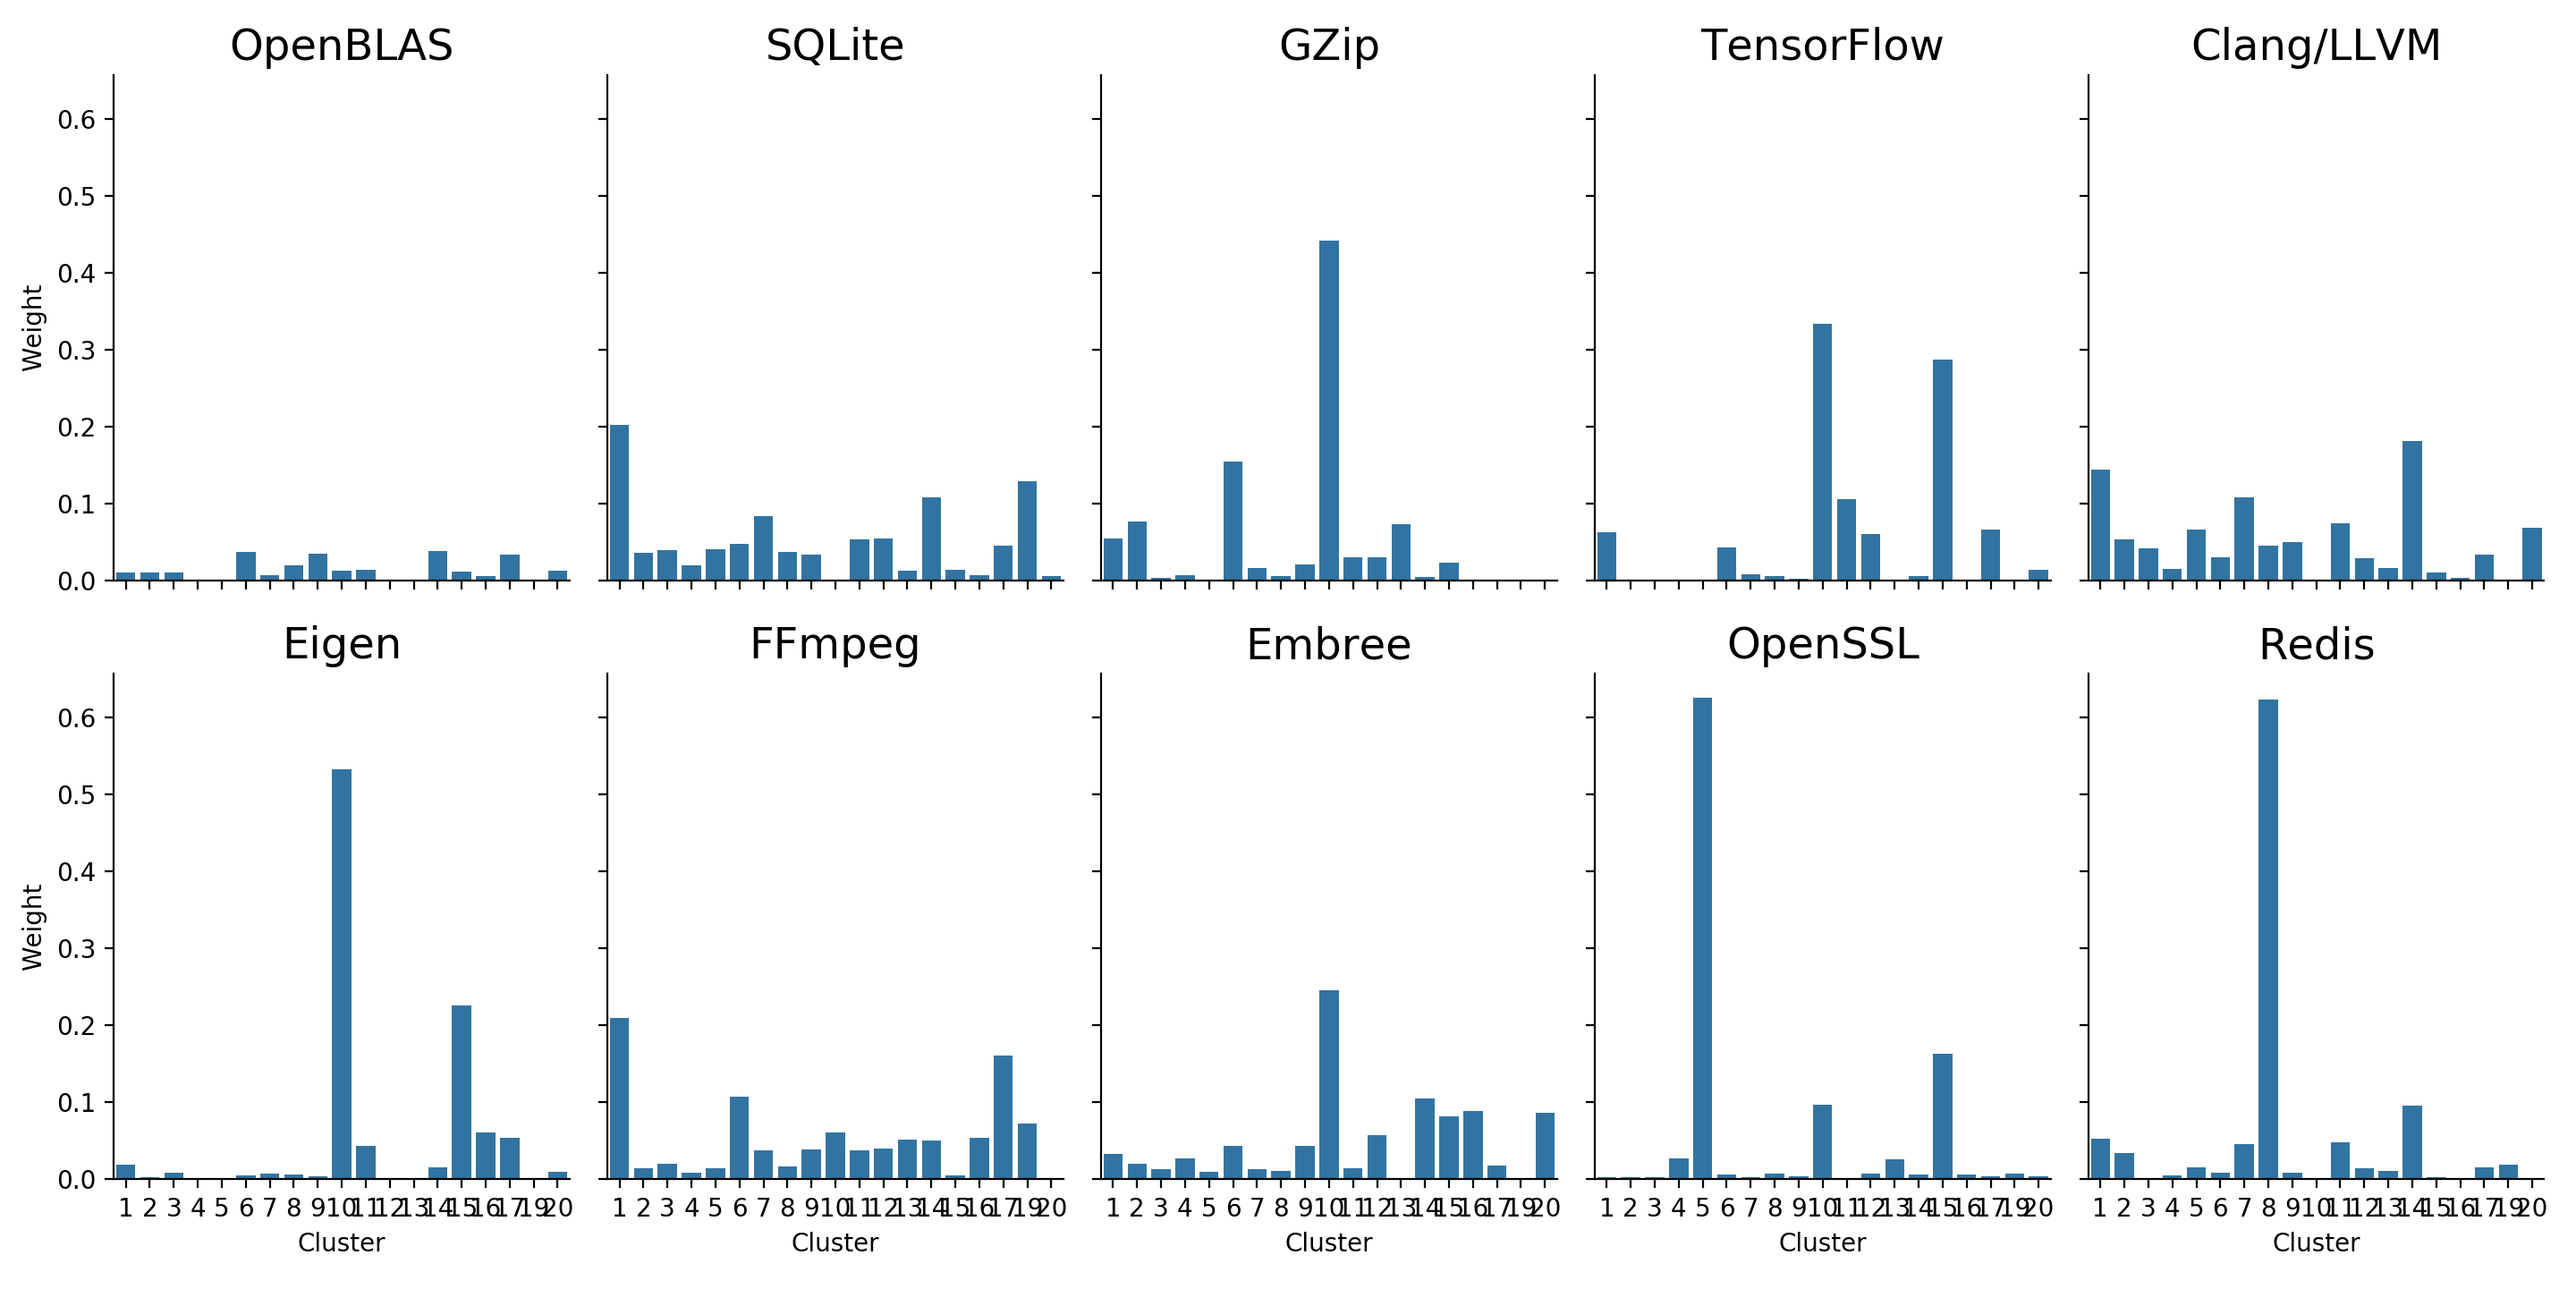
\includegraphics[width=\textwidth]{figures/apps-vs-clusters.png}
\caption{Breakdown of applications by basic block classes.
Y-axis represents the total weight of basic blocks
in a given class.
Cluster-16 contains vectorized basic blocks.
Note that the breakdown of OpenBLAS can be surprising
because the official benchmark contains
unoptimized verification code that got included into
our analysis}
\label{fig:apps_vs_clusters}
\end{figure*}
